\documentclass[12pt, a4]{article}
\usepackage[english]{babel}
\usepackage[utf8x]{inputenc}
\usepackage{fullpage}
\usepackage{listings}
\usepackage{graphicx}
\usepackage{color}

%Syntax highlighting
\definecolor{blue-violet}{rgb}{0.54, 0.17, 0.89}
\definecolor{ao}{rgb}{0.0, 0.5, 0.0}
\definecolor{amaranth}{rgb}{0.9, 0.17, 0.31}
\definecolor{ballblue}{rgb}{0.13, 0.67, 0.8}
\definecolor{onyx}{rgb}{0.06, 0.06, 0.06}


\lstset{
  breaklines=true,                 % automatic line breaking only at whitespace
  captionpos=b,                    % sets the caption-position to bottom
  breakatwhitespace=false,
  keepspaces=true,
  numbers=left,
  numbersep=5pt,
  showspaces=false,
  showstringspaces=false,
  showtabs=false,
  tabsize=4,  
  backgroundcolor=\color{white},   % choose the background color
  commentstyle=\color{ao},    % comment style
  keywordstyle=\color{amaranth},    % keyword style
  stringstyle=\color{blue-violet},    % string literal style
  numberstyle=\tiny\color{ballblue},	   % number style
  basicstyle=\ttfamily\footnotesize\color{onyx} % size of fonts used for the code
}

%Document Header
\title{\textbf{Department of CSE\\SSN College of Engineering}}
\author{\textbf{Vishakan Subramanian - 18 5001 196 - Semester VII}}
\date{14 September 2021}

\begin{document}
\maketitle
\hrule
\section*{\center{UCS 1712 - Graphics And Multimedia Lab}}
\hrule
\bigskip

%Assignment Details
\subsection*{\center{\textbf{Exercise 8: 3D Transformations in C++ using OpenGL}}}
\subsection*{\flushleft{Aim:}}
\begin{flushleft}

To apply the following 3D transformations on objects and to render the final output along with the
original object.

\begin{itemize}
	\item Translation
	\item Rotation
	\item Scaling
	\item Reflection
	\item Shearing 
\end{itemize} 

\bigskip
Display the original and the transformed object.
 
\end{flushleft}

%Code
\newpage
\subsection*{\flushleft{Code: 3D Transformations:}}
\begin{flushleft}
\lstinputlisting[language = C++]{3DTransforms.cpp}
\end{flushleft}


%Output
\newpage
\subsection*{\flushleft{Output: Base 3D Object}}
\begin{figure}[h]
\centering
\caption{Base 3D Object.}
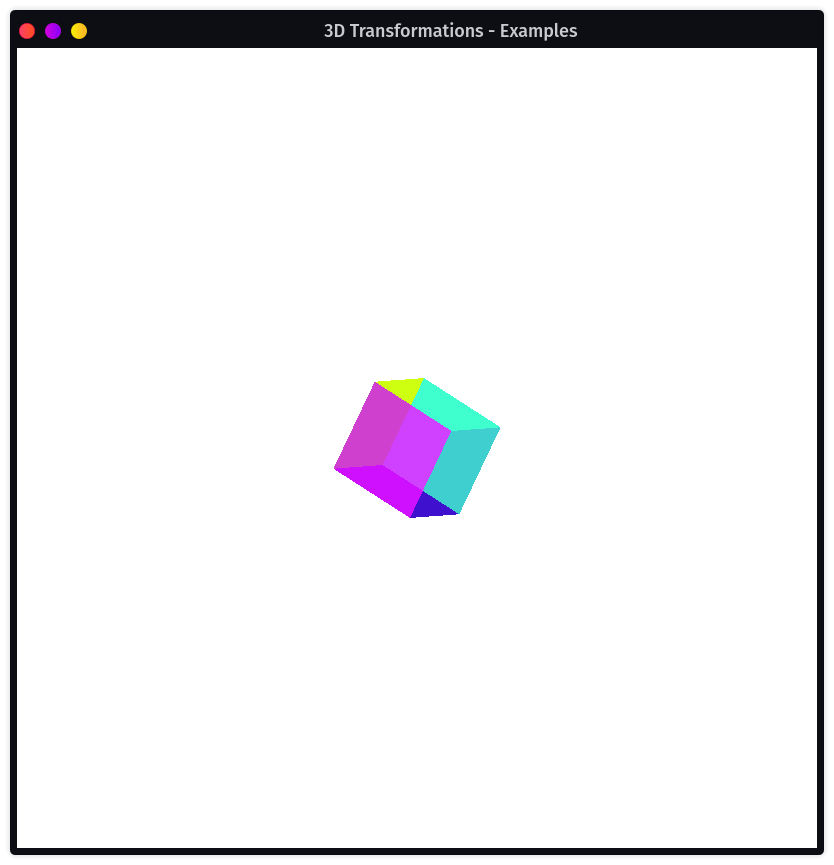
\includegraphics[height=15cm, width=15cm]{Outputs/Output-0.png}
\end{figure}

%Output
\newpage
\subsection*{\flushleft{Output: Console - Translation, (200, 300, 400)}}
\begin{figure}[h]
\centering
\caption{Output: Console - Translation, (200, 300, 400).}
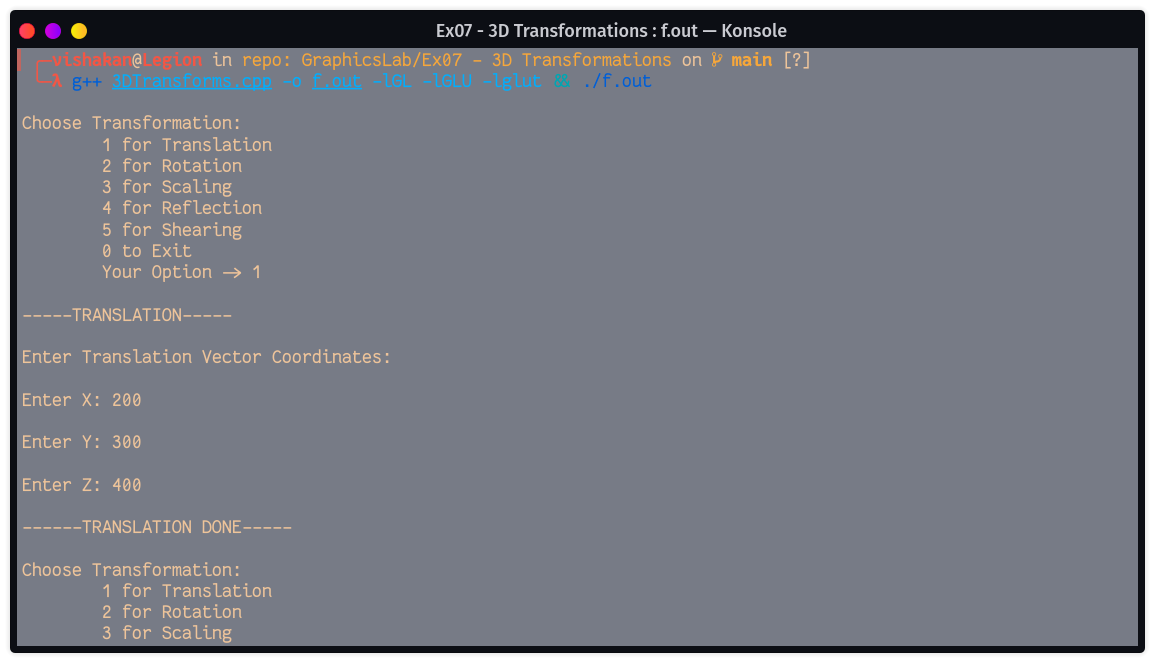
\includegraphics[height=12cm, width=17cm]{Outputs/Console-1.png}
\end{figure}

%Output
\newpage
\subsection*{\flushleft{Output: Translated 3D Object, (200, 300, 400)}}
\begin{figure}[h]
\centering
\caption{Translated 3D Object, (200, 300, 400).}
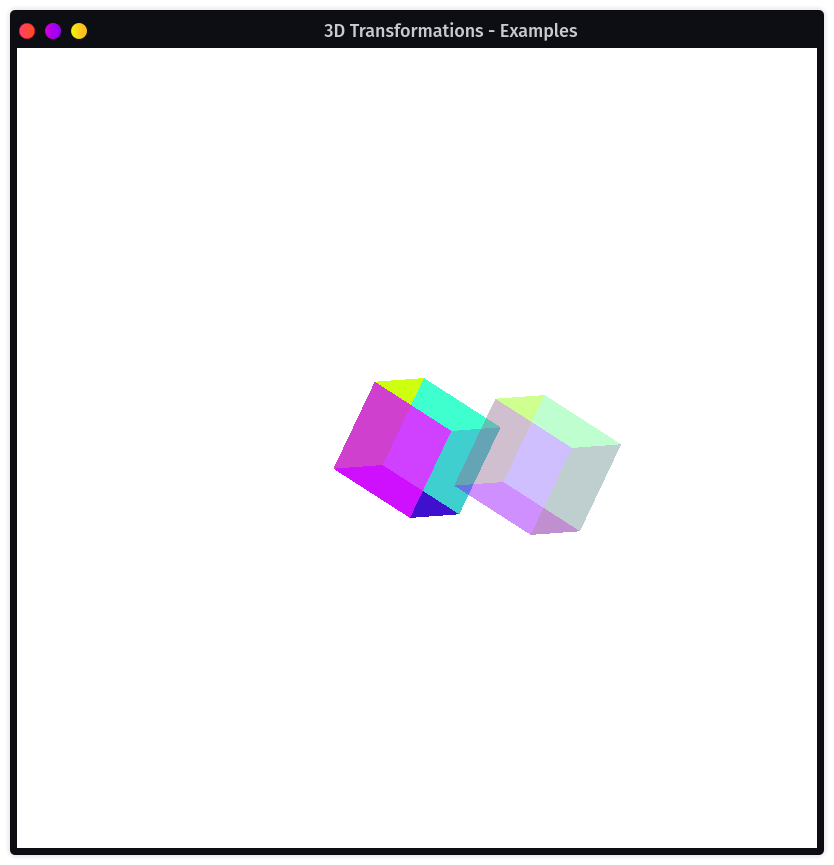
\includegraphics[height=15cm, width=15cm]{Outputs/Output-1.png}
\end{figure}

%Output
\newpage
\subsection*{\flushleft{Output: Console - Rotation, Y-Axis, $120^{\circ}$}}
\begin{figure}[h]
\centering
\caption{Output: Console - Rotation, Y-Axis, $120^{\circ}$.}
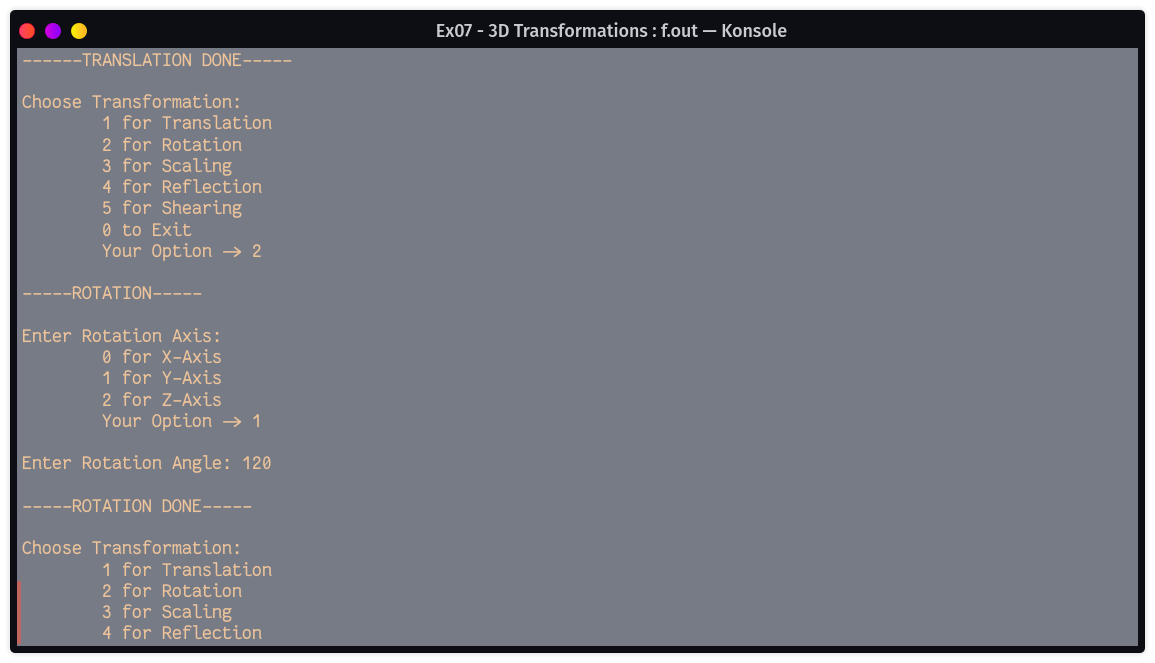
\includegraphics[height=12cm, width=17cm]{Outputs/Console-2.png}
\end{figure}

%Output
\newpage
\subsection*{\flushleft{Output: Rotated 3D Object, Y-Axis, $120^{\circ}$}}
\begin{figure}[h]
\centering
\caption{Rotated 3D Object, Y-Axis, $120^{\circ}$.}
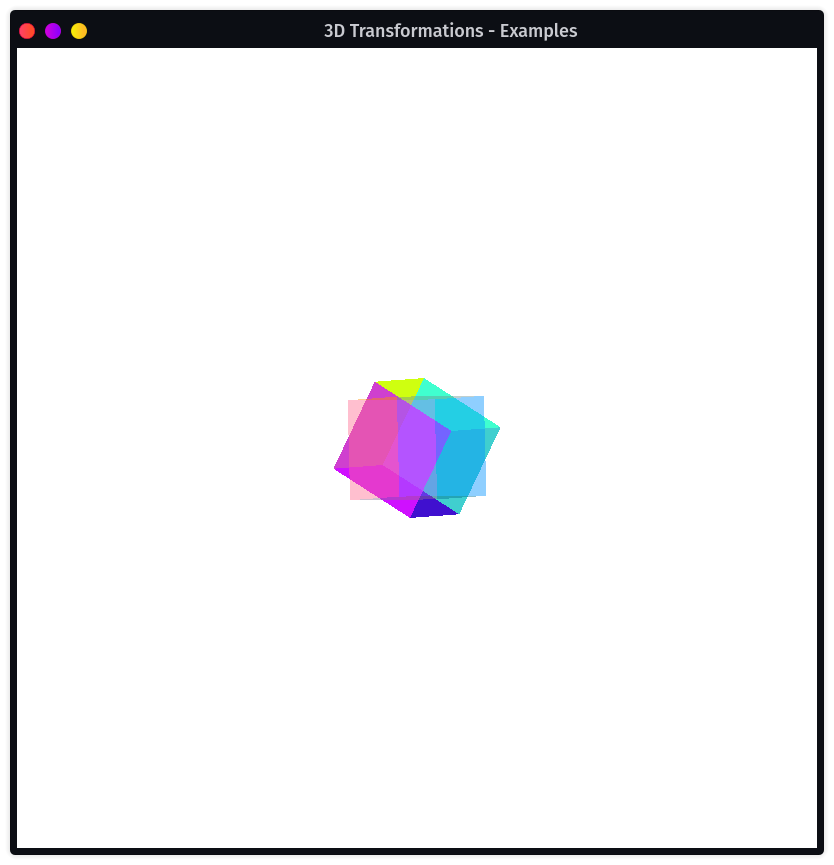
\includegraphics[height=15cm, width=15cm]{Outputs/Output-2.png}
\end{figure}

%Output
\newpage
\subsection*{\flushleft{Output: Console - Scaling, (2, 1.5, 3)}}
\begin{figure}[h]
\centering
\caption{Output: Console - Scaling, (2, 1.5, 3).}
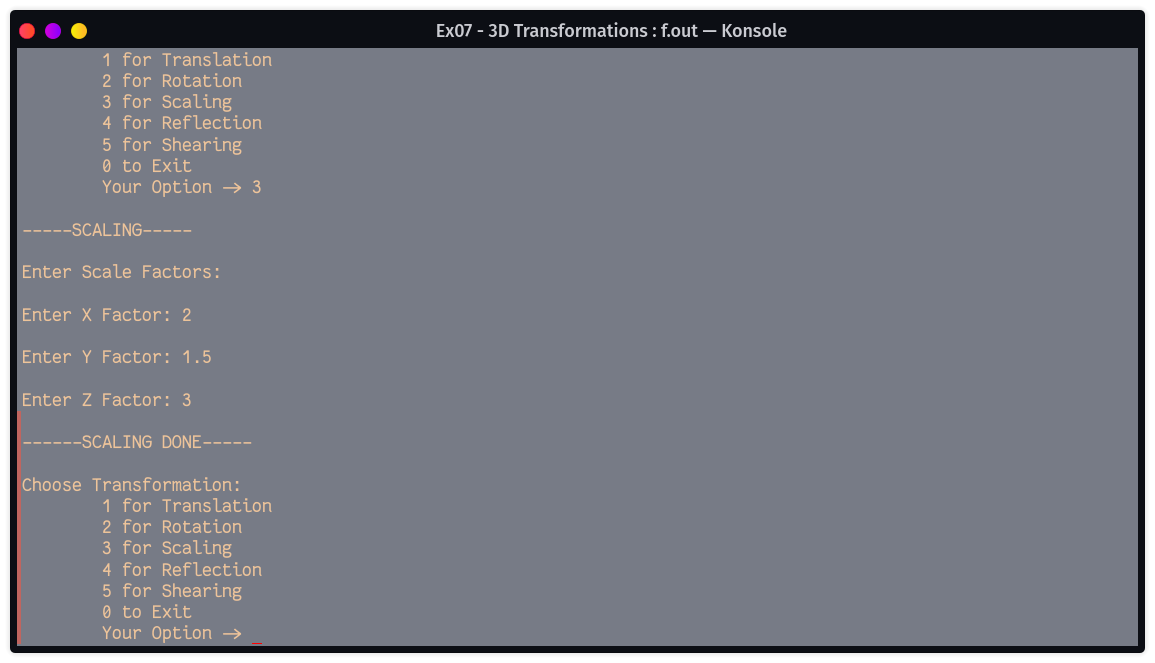
\includegraphics[height=12cm, width=17cm]{Outputs/Console-3.png}
\end{figure}

%Output
\newpage
\subsection*{\flushleft{Output: Scaled 3D Object, (2, 1.5, 3)}}
\begin{figure}[h]
\centering
\caption{Scaled 3D Object, (2, 1.5, 3).}
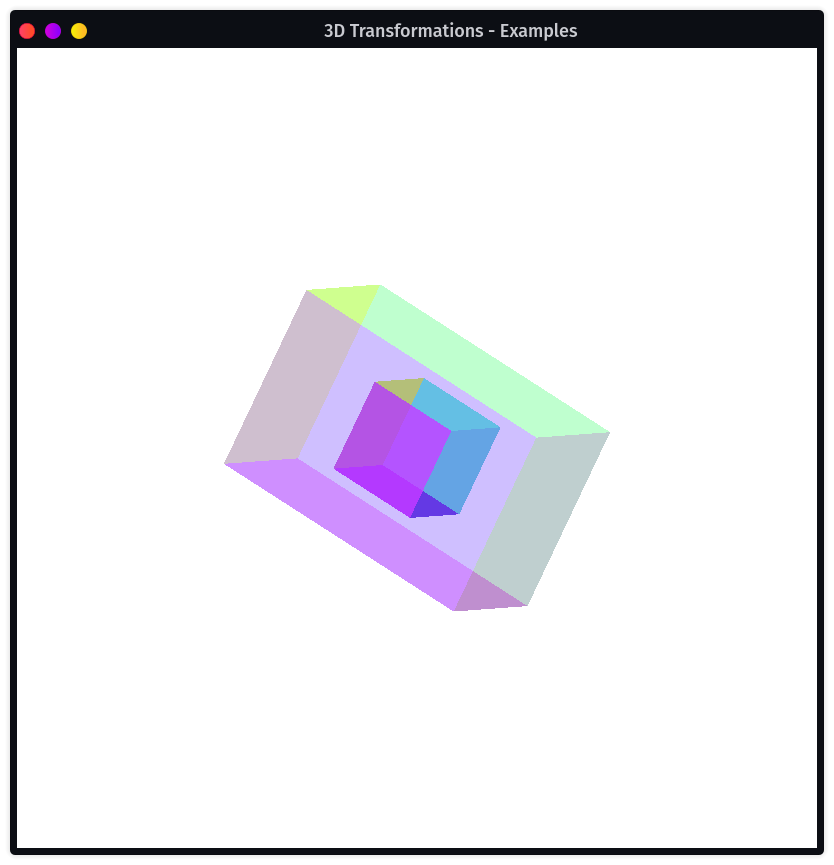
\includegraphics[height=15cm, width=15cm]{Outputs/Output-3.png}
\end{figure}

%Output
\newpage
\subsection*{\flushleft{Output: Console - Reflection, ZX Plane}}
\begin{figure}[h]
\centering
\caption{Output: Console - Reflection, ZX Plane.}
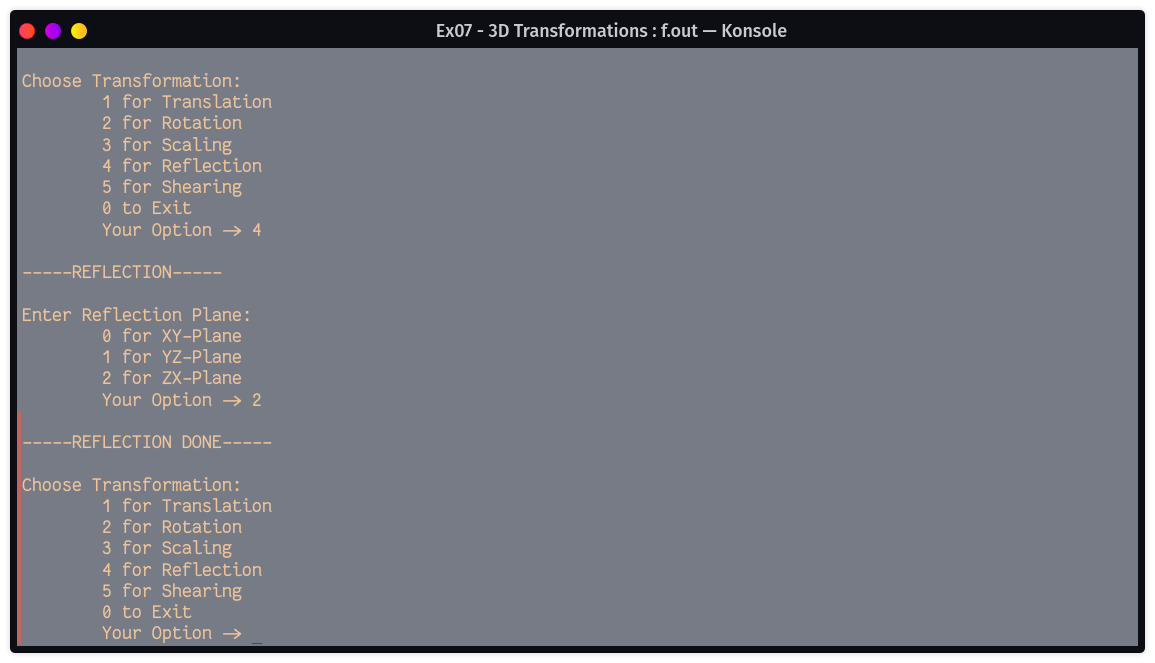
\includegraphics[height=12cm, width=17cm]{Outputs/Console-4.png}
\end{figure}

%Output
\newpage
\subsection*{\flushleft{Output: Reflected 3D Object, ZX Plane}}
\begin{figure}[h]
\centering
\caption{Reflected 3D Object, ZX Plane.}
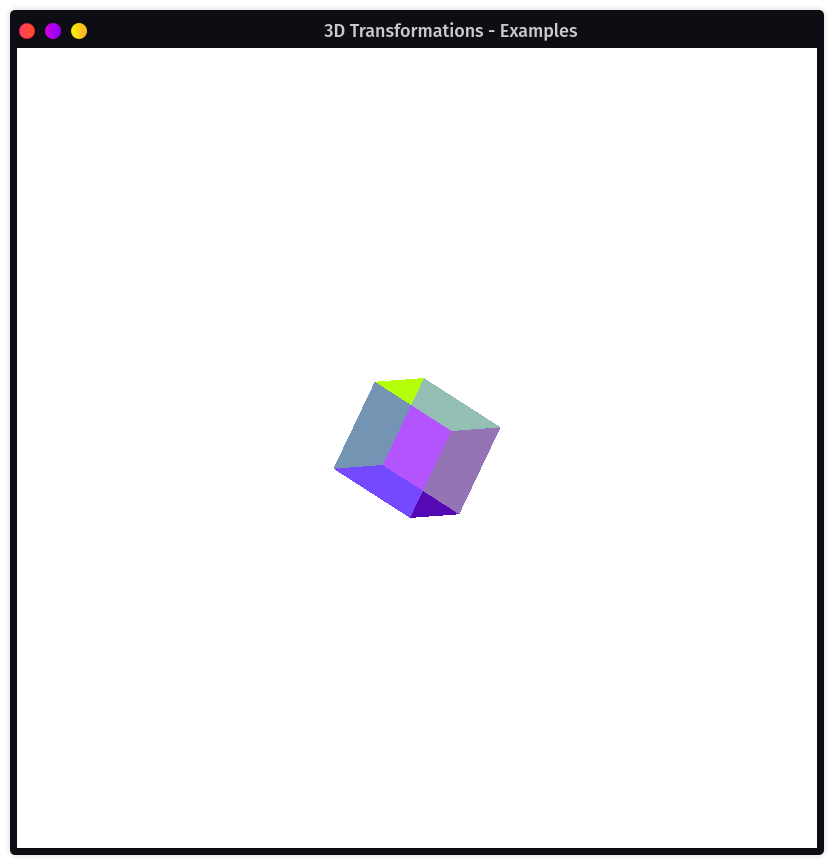
\includegraphics[height=15cm, width=15cm]{Outputs/Output-4.png}
\end{figure}

%Output
\newpage
\subsection*{\flushleft{Output: Console - Shearing, X Axis, (2.5, 3)}}
\begin{figure}[h]
\centering
\caption{Output: Console - Shearing, X Axis, (2.5, 3).}
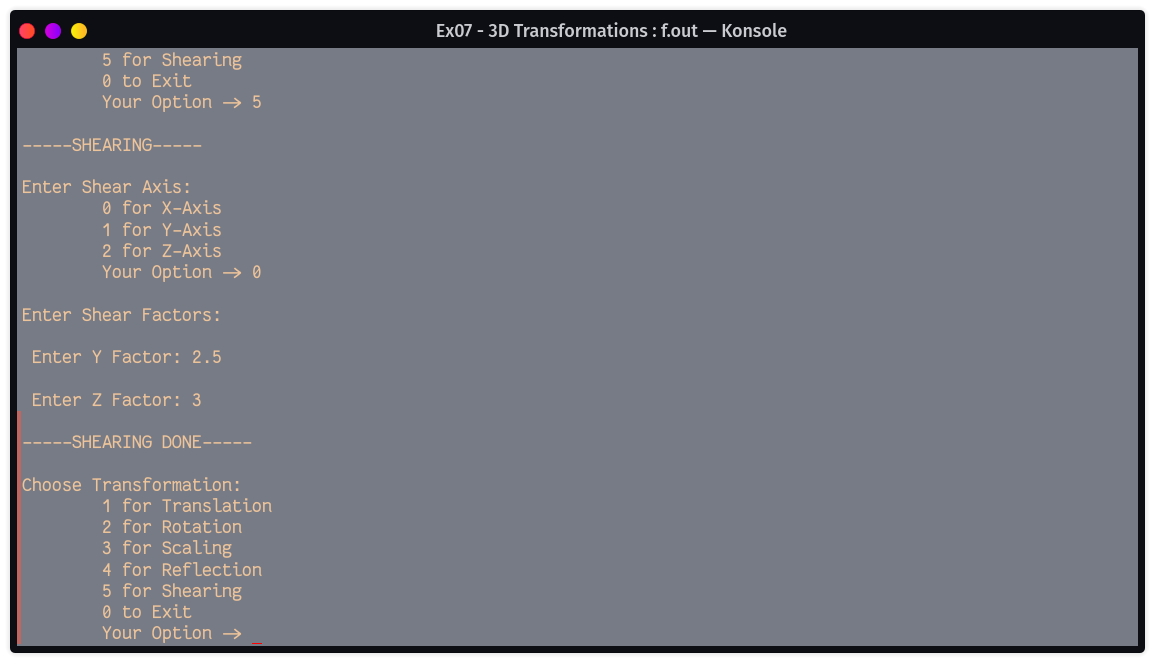
\includegraphics[height=12cm, width=17cm]{Outputs/Console-5.png}
\end{figure}

%Output
\newpage
\subsection*{\flushleft{Output: Sheared 3D Object, X Axis, (2.5, 3)}}
\begin{figure}[h]
\centering
\caption{Sheared 3D Object, X Axis, (2.5, 3).}
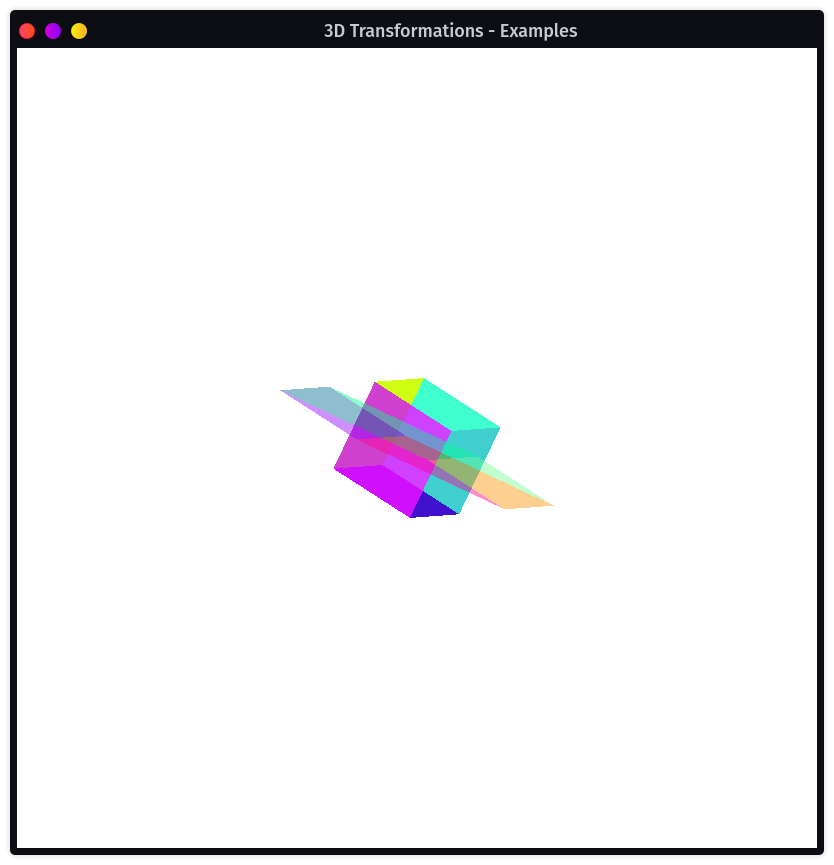
\includegraphics[height=15cm, width=15cm]{Outputs/Output-5.png}
\end{figure}




%Learning Outcome
\newpage
\subsection*{\flushleft{Learning Outcome:}}
\begin{itemize}
\item I learnt how to represent a \textbf{3D Object} in terms of its \textbf{2D Faces} as planar polygons.
\item I learnt how to perform \textbf{Translation, Rotation, Scaling, Reflection and Shearing} upon a given 3D Object with the use of 3D transformation matrices.
\item I learnt about the different transformation matrices and how to calculate them.
\item I learnt how to set \textbf{depth flags} to enable the \textbf{Z-Axis} projections.
\item I came to know about inbuilt functions that perform the same transformations like \textbf{glRotate3f()} in OpenGL.
\item I learnt how to do \textbf{orthographic projection} in 3D with OpenGL, using \textbf{glOrtho()}.
\item I learnt to use parametrized and default constructors in C++ and to call them from other constructors.
\end{itemize}


\end{document}